\documentclass[../portafolio.tex]{subfiles}

% Solo agregue paquetes en el preámbulo de ../portafolio.tex

\begin{document}

\chapter{Instrucciones generales}
\label{ch:instrucciones}

\chapterauthor{Roberto E. Navarro}
%%%%%%%%%%%%%%%%%%%%%%%%%%%%%%%%%%%%%%%%%%%%%%%%%%%%%%%%%%%%%%%%%%%%%%%%%%%%%%%%

\hfill \textbf{Fecha de la actividad:} 23 de septiembre de 2025

\medskip

\textcolor{red}{\bf Elimine este capítulo de su portafolio}.

\medskip

Este capítulo presenta instrucciones generales para la correcta
preparación y presentación de su portafolio, incluyendo ejemplos
prácticos de ecuaciones, figuras, códigos y referencias en \LaTeX.

Las evidencias de aprendizaje en este documento consistirán en la
entrega de soluciones detalladas a problemas específicos seleccionados
durante la asignatura. Cada problema o evidencia debe ser presentado en un capítulo distinto, y estos deberán incluir:
%
\begin{description}
\item[Título del capítulo] Un título adecuado que describa breve y claramente de qué trata el capítulo. Evite títulos como ``Problema 3'' o ``Tarea 2''. Sea explícito, por ejemplo: ``Resolución numérica de la ecuación de onda unidimensional'' o ``Simulación de un péndulo amortiguado con el método de Runge-Kutta de cuarto orden''.
\item[Autor(es)] El autor o autores del capítulo, separados por coma. Use al menos un nombre y un apellido por autor.
\item[Fecha] La fecha de entrega del capítulo. Prefiera el formato ``[día] de [mes] de [año]''.

\item[Resumen y objetivos] Presente el problema en sus propias
  palabras, parafraseando el enunciado de la guía en lugar de copiarlo
  textualmente. Explique claramente cuáles son los objetivos del
  problema y describa brevemente cómo planea abordarlo.

\item[Desarrollo del problema] Explique con sus propias palabras cómo
  resolvió el problema. No se limite a mostrar solo fórmulas o código:
  describa el procedimiento seguido, los pasos intermedios y las
  decisiones tomadas.  Si se requiere demostrar un esquema numérico,
  detalle el razonamiento utilizado. En problemas numéricos, indique
  qué algoritmo o enfoque usó, incluyendo fragmentos de código en
  \lstinline!python! que sean relevantes (por ejemplo, funciones o
  implementaciones de esquemas), pero \textbf{no copie el código
    completo}. Omita líneas triviales como importación de librerías o
  configuración de gráficos. Puede citar los códigos de python alojados en la carpeta \lstinline!src/!.

  Interprete los resultados obtenidos en lugar de solo
  mostrarlos. Discuta su significado y validez: ¿aparecen errores
  numéricos?, ¿la aproximación es adecuada? ¿los resultados obtenidos coinciden con lo esperado?, ¿qué muestran los gráficos
  o tablas? Incluya la reflexión necesaria para conectar los
  resultados con los objetivos del problema, citando referencias si es
  pertinente.

\item[Conclusiones] Al final de cada capítulo, presente un resumen
  breve de lo realizado y de los resultados más relevantes. No se
  limite a repetir el enunciado del problema o el procedimiento:
  explique qué aprendió al resolverlo, las dificultades que enfrentó y
  cómo las superó. Finalmente, reflexione sobre cómo este problema en
  particular aporta a su comprensión de los métodos computacionales en
  física.

\item[Agradecimientos] En capítulos con más de un autor, declare la
  participación de cada autor. Por ejemplo, ¿quiénes desarrollaron la
  solución?  ¿quién redactó el capítulo? ¿quién elaboró las figuras y
  tablas?  ¿quién escribió los códigos de python? ¿quién revisó la
  integridad del capítulo? ¿Hubo dificultades en la coordinación del
  grupo?.

  Si corresponde, incluya una breve nota de
  agradecimiento a personas externas al grupo que lo apoyaron en la resolución de
  esta actividad. Además, declare de forma explícita si utilizó o no
  herramientas de inteligencia artificial en la elaboración de su
  trabajo, especificando en qué aspectos fueron usadas (por ejemplo,
  redacción del texto, demostración de un esquema numérico,
  elaboración o depuración de código, etc.).
\end{description}

A continuación se presenta una breve guía de elementos que puede usar en \LaTeX\ para cuidar la presentación del mismo. Luego, en el capítulo \ref{ch:ejemplo-derivadas}, mostramos un ejemplo de un problema que incorpora los elementos esperados en cada capítulo.


%---------------------------------------------------------------------------------
\section{Ecuaciones}

Dependiendo de su estilo, puede utilizar ecuaciones dentro del texto como
$f(x)=\frac{x}{\sqrt{1-x^2}}$.

\subsection{Ecuaciones largas}
Si la ecuación es larga o es importante (aunque no sea tan larga),
debería dedicar una línea solo para esa ecuación. Así, para ecuaciones
que son claramente relevantes, debe enumerarlas usando
\lstinline[language=TeX]!equation!. Por ejemplo,
\begin{equation}
  \label{eq:euler}
\exp(i\theta) = \cos\theta + i\sin\theta \,.
\end{equation}

Si la ecuación es parte de un procedimiento, debe usar \lstinline[language=TeX]!align!. Por ejemplo,
\begin{align}
  \frac{d}{dx} x^2 \sin x
  &= \left(\frac{dx^2}{dx}\right)  \sin x + x^2 \frac{d}{dx} \sin x \,, \nonumber \\
  &= 2x \sin x + x^2 \cos x \,. \label{eq:regla-producto}
\end{align}

Note el uso de \lstinline[language=TeX]!\nonumber! para eliminar la enumeración de una
línea. Note también el uso de puntos y comas en las ecuaciones
\eqref{eq:euler} a \eqref{eq:regla-producto}.

Evite rayar ecuaciones con líneas oblicuas, tachaduras o llaves
horizontales para indicar qué términos se anulan o qué parte
corresponde a cierta operación. Aunque pueda parecer útil en
borradores a mano, en un documento final estas marcas recargan el
texto y dificultan la lectura. Prefiera la explicación en prosa. Es
más limpio y profesional escribir, por ejemplo \textit{``Al anularse
  el término lineal, la ecuación se reduce a...''}  en lugar de tachar
el término dentro de la expresión.

Evite también símbolos innecesarios como $\Rightarrow$, $\therefore$ o
$\Leftrightarrow$. En la mayoría de los casos, estos símbolos no
agregan información adicional y podrían ensuciar la presentación o
terminar confundiendo más de lo que aclaran. Si siente la necesidad de
hacer un truco tipográfico (como rayas, flechas improvisadas, etc.),
que usualmente requieren comandos de \LaTeX\ poco comunes o sintaxis
enrevesada que dificulta la lectura de las fuentes en \LaTeX,
probablemente sea señal de que lo mejor es reescribir la
explicación. Un párrafo bien redactado no solo transmite mejor la
idea, sino que también hace que el documento se lea con fluidez, luzca
profesional y resulte más sencillo de depurar y editar en el código
fuente.

\subsection{Referencia a ecuaciones}


Puede citar ecuaciones enumeradas, por ejemplo la ecuación
\eqref{eq:euler} tiene la etiqueta \lstinline[language=TeX]!eq:euler!, configurado con el comando \lstinline[language=TeX]!\label{eq:euler}! y citado con el el comando \lstinline[language=TeX]!\eqref{eq:euler}!.

Como recomendación general, la etiqueta debería ser una palabra que
claramente identifique al objeto que queremos citar (por ejemplo,
\lstinline[language=TeX]!eq:euler! claramente se refiere a la ecuación
de Euler). No use etiquetas numéricas como
\lstinline[language=TeX]!\label{eq:1}! porque es muy posible que el
número de ecuación cambie en el futuro y haga que usted se confunda.

De la misma forma, note que podemos hacer referencias a ecuaciones de
otros capítulos, a figuras, tablas, capítulos y secciones. Por ejemplo, en la
sección \ref{sec:figuras}
(\lstinline[language=TeX]!\ref{sec:figuras}!) discutiremos cómo
incluir figuras.

\section{Figuras} \label{sec:figuras}
También puede agregar figuras para explicar mejor sus ideas. Trate de
citarlas adecuadamente en el texto, por ejemplo, la figura
\ref{fig:estatica} (\lstinline[language=TeX]!\ref{fig:estatica}!) muestra un ejemplo usado en wikipedia
para explicar la electricidad estática~\citep{wikistatic}.
\begin{figure}[ht!]
  \centering
  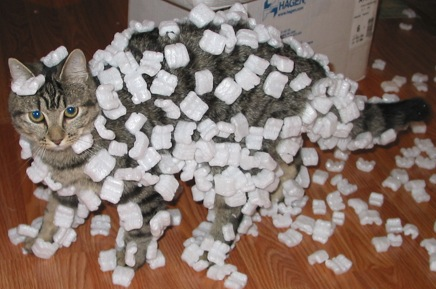
\includegraphics[width=0.5\textwidth]{static_cat_wikipedia}
  \caption{Bolas de poliestireno adheridos al pelaje de un gato debido
    a la electricidad estática~\citep{wikistatic}.}
  \label{fig:estatica}
\end{figure}

En este caso, citamos la figura usando el comando \lstinline[language=TeX]!\ref{fig:estatica}!. No es una buena práctica tratar de referirse a una figura como ``la siguiente figura'' porque estas tienden a moverse en el texto para aprovechar mejor los espacios. \textcolor{red}{\bf NO INTENTE FORZAR LA POSICIÓN DE UNA FIGURA}. O sea, \textbf{nunca} use \lstinline[language=TeX]![H]! para que la figura aparezca donde usted quiere. Deje que la figura sea libre y que \LaTeX\ decida dónde queda mejor. Por ejemplo, es posible que la figura~\ref{fig:estatica} se encuentre en otra página en la compilación de este documento. Pero no importa, porque usted sabe que nos estamos refiriendo a la figura~\ref{fig:estatica} y no a otra cosa.


\section{Códigos}
Puede incluir códigos usando el paquete
\lstinline[language=TeX]!listings!. Para incluir código de python, por
ejemplo, para mostrar cómo calcular la derivada centrada de una serie
ordenada de puntos $(x_i,\,y_i)$ usando un ciclo
\lstinline[language=TeX]!for!, use la siguiente sintaxis:
\begin{lstlisting}[language=TeX,escapechar=@]
\begin{@@lstlisting}
for i in range(1,y.size-1):
    dy[i] = (y[i+1]-y[i-1]) / (x[i+1]-x[i-1])
\end{@@lstlisting}
\end{lstlisting}

En este caso, le indicamos a \lstinline!lstlisting! que queremos usar colores especiales para el lenguaje \lstinline!python! (configurado por defecto en este portafolio). Puede usar otros estilos usando la opción \lstinline!language!, por ejemplo \lstinline!\begin{lstlisting}[language=TeX]!. Vea la \href{https://ctan.org/pkg/listings}{documentación oficial} o la \href{https://www.overleaf.com/learn/latex/Code_listing}{guía de overleaf} para más ejemplos y lenguajes soportados.



\section{Referencias bibliográficas}
Al final del documento encontrará una lista de referencias. Esto se logra usando \lstinline[language=TeX]!bibtex! y el archivo \lstinline[language=Bash]!referencias.bib! que se encuentra en el directorio base de este portafolio.

El archivo \lstinline[language=Bash]!referencias.bib! tiene entradas de la forma:
\begin{lstlisting}[language=TeX]
@misc{wikistatic,
    author = "{Wikipedia contributors}",
    title = "Static electricity --- {Wikipedia}{,} The Free Encyclopedia",
    year = "2021",
    howpublished = {\url{https://en.wikipedia.org/w/index.php?title=Static...}},
    note = "[Online; accessed 5-November-2021]"
  }
\end{lstlisting}

En este caso, es una referencia a una página web y es de tipo \lstinline[language=TeX]!@misc!, donde la primera palabra \lstinline[language=TeX]!wikistatic! es la etiqueta que usamos para citar, y las entradas \lstinline[language=TeX]!author!, \lstinline[language=TeX]!title!, etc. son información que \lstinline!bibtex! usa para formatear la bibliografía al final del documento.

Para citar esta referencia en el texto, usamos el comando \lstinline[language=TeX]!\citep{wikistatic}!. Puede citar más referencias separándolas con comas, por ejemplo \lstinline[language=TeX]!\citep{wikistatic,AF:2003,CEL:arXiv}! que resulta en \citep{wikistatic,AF:2003,CEL:arXiv}. Note que existen tres comandos disponibles \lstinline[language=TeX]!\cite!, \lstinline[language=TeX]!\citet! y \lstinline[language=TeX]!\citep!. Abajo explico un poco más.

Para compilar este documento (si es que está trabajando localmente en su computador con \LaTeX\ instalado), recomiendo usar el comando \lstinline[language=Bash]!latexmk!:
\begin{lstlisting}[language=Bash]
latexmk -pdf portafolio.tex
\end{lstlisting}

Esto asegura la correcta compilación de todos los elementos del
documento, incluyendo referencias cruzadas a figuras y ecuaciones,
además de citas bibliográficas. La etiqueta \lstinline[language=Bash]!-pdf! es para compilar el documento en formato PDF.

El comando \lstinline!latexmk! es capaz de reconocer si su documento requiere o no una nueva compilación, para lo cual crea archivos auxiliares. A veces, estos archivos auxiliares se corrompen, por lo que si usted obtiene un error de compilación, le sugiero eliminarlos con la opción \lstinline!-C!:
\begin{lstlisting}[language=Bash]
latexmk -pdf -C portafolio.tex
\end{lstlisting}


Si tiene algún problema con la bibliografía, es posible que no tenga algunos elementos instalados (como la librería \lstinline[language=Bash]!texlive-publishers!). Busque en \lstinline[language=Bash]!portafolio.tex! la siguiente línea para diagnosticar el problema:
\begin{lstlisting}[language=TeX]
% % bibliografia: descomente estas dos lineas para usar estilo numerico, e.g. [1].
% \usepackage[square,numbers,sort&compress]{natbib}
% \bibliographystyle{apsrev4-1}

% bibliografia: descomente estas dos lineas para usar estilo autor-año,
% e.g. (Navarro, 2022).
\usepackage[authoryear]{natbib}
\bibliographystyle{aipauth4-1}
...
% lista de referencias guardadas en referencias.bib
\bibliography{referencias}

\end{document}
\end{lstlisting}

En el texto anterior, \lstinline[language=TeX]!\bibliographystyle! controla el estilo de bibliografía. Por ejemplo,
\begin{itemize}
\item El estilo \lstinline[language=TeX]!apsrev4-1! configurado con \lstinline[language=TeX]!square,numbers,sort\&compress! resulta en referencias numéricas:
\begin{lstlisting}[language=TeX]
\cite{CEL:arXiv}  : [3]
\citep{CEL:arXiv} : [3]
\citet{CEL:arXiv} : Cancès et al. [3]
\end{lstlisting}

\item El estilo \lstinline[language=TeX]!aipauth4-1! configurado con \lstinline[language=TeX]!authoryear! resulta resulta en referencias autor-año:
\begin{lstlisting}[language=TeX]
\cite{CEL:arXiv}  : Cancès, Ehrlacher, and Lelièvre (2012)
\citep{CEL:arXiv} : (Cancès, Ehrlacher, and Lelièvre, 2012)
\citet{CEL:arXiv} : Cancès, Ehrlacher, and Lelièvre (2012)
\end{lstlisting}
\end{itemize}


\section{Comentarios finales}

Note que \textbf{cada capítulo se puede compilar independientemente del portafolio}. Esto es posible gracias al paquete \lstinline[language=TeX]!subfiles!.

Al principio de este archivo (\lstinline!instrucciones.tex!), encuentra la instrucción
\begin{lstlisting}[language=TeX]
\documentclass[../portafolio.tex]{subfiles}
\end{lstlisting}

Esto significa que este archivo hereda los paquetes y algunas configuraciones del archivo principal \lstinline[language=TeX]!../portafolio.tex!.

Para compilar este capítulo y solo este capítulo, puede usar:
\begin{lstlisting}[language=Bash]
latexmk -pdf instrucciones.tex
\end{lstlisting}

Como no incluimos \lstinline[language=TeX]!\bibliography{referencias}! en este documento, es posible que las referencias bibliográficas no se resuelvan bien. Además, si cita ecuaciones o figuras de otros capítulos tampoco se resolverán, apareciendo un símbolo como \lstinline[language=TeX]!(??)!. Pero esto no importa, pues la utilidad de esto es solo  compilar este documento de forma rápida para diagnosticar como se está viendo. Una vez este capítulo esté finalizado, puede compilar el portafolio completo y las referencias estarán bien resueltas.
\end{document}
